\section{Experimental Study}
\label{sec:exp}
%\subsection{Implementation Issues}
%We use Apache Spark~\footnote{http://spark.apache.org/} as the experimental
%platform. Spark is one of the most popular MapReduce platform which
%uses in-memory cache to gain high speedup against Apache Hadoop~\cite{}. 
%Due to the direct support of MapReduce, our algorithm can be easily implemented in Spark. 
%In order to help reproduce our experiments, we further address some implementation issues.
%\subsubsection{Task Assignment}
%In spark, each task in reduce phase is an Apriori mining phase of 
%a star.
%Although our star partition method is theoretically balanced, 
%it is still necessary to assign equal number of tasks to each executors. 
%Spark naturally uses hashing to partition data into tasks, where such
%a partitioning does not care on the tasks size. In order to
%fully utilize the clusters, it is important to perform a weight-aware
%partition. In our implementation, we collect the number of edges
%in each star after map phase. Afterwards, we use a simple \emph{best-fit} strategy,
%where we assign stars in decreasing order with their sizes and each star
%is assigned to the currently least-loaded executor.  HERE WE MAY HAVE ANOTHER BOUND
%FROM LITERATURE, BUT I DIDN'T FIND YET. The injection of load balancing strategy
%between map and reduce phase can be naturally implemented in Spark, where the 
%map result can be cached and the reduce phase can be paused until when the
%partition strategy is ready.
%
%\subsubsection{Duplication Detection}
%It is notable that the patterns discovered from different tasks (stars) could
%be redundant due to containment relationship. For example, a pattern $\{a,b,c\}$
%can be discovered from the star $Sr_a$, while the pattern $\{b,c\}$ can be discovered
%from the star $Sr_b$. Though in most applications, such a duplicate pattern
%is permitted, we offer an option to eliminate these patterns. The strategy is 
%to broadcast each reducers output to every other reducers. This can be
%efficiently done via \emph{broadcast} variables~\footnote{http://spark.apache.org/docs/latest/programming-guide.html\#broadcast-variables} in Spark. Afterwards, each reduce can check 
%whether any resulted patterns are subsumed and thus filter those patterns.
%Theoretically, advanced techniques, such as Bloom Filters, can be applied to efficiently
%deal with the duplication detection. However, as the number of final patterns are
%normally quit small, we leave the exploration for those techniques to the future.
%
%\subsubsection{Handling Overlapping Clusters}
%When handling patterns such as \emph{flock} and \emph{group}, disk-based clustering
%on objects are applied. Such a clustering method may result one object belonging to
%multiple clusters. In such a case, just keeping the timestamps in the edge
%of connection graph is insufficient. Instead, we extend every timestemp $t$
%to a pair $\langle t,C \rangle$, where $C$ is the set of clusters objects
%belong to at time $t$. The only adaption we need to take the join during
%apriori phase. Given two timestamp set $T_1$ and $T_2$, the join result of
%$T_1$ and $T_2$ instead of being $\{\forall t | t\in T_1 \wedge t_\in T_2\}$,
%it changes to $\{\forall (t,C) | t\in T_1 \wedge t \in T_2 \wedge C = (T_1.C \cap T_2.C) \wedge C \neq \emptyset\}$.
%It is obvious to see the \emph{edge simplification} and \emph{candidate pruning} 
%still holds under this new setting.


\subsection{Experimental Setup}
We adapt one of the most popular MapReduce platform, Apache Spark, 
to conduct experiments on mining GCMPs. 
Our experiments run on a 9-node cluster, with Apache Yarn as
the cluster manager. We use 1 node for Yarn resource manager, 
and use the remaining 8 nodes as executors. Each node in the cluster
is uniformly equipped with a 2.2GHz quad-core CPU with 32 GB memory. 
Inter-node communication is carried by 
the 1Gbps Ethernet.  Some critical configuration of Spark is 
as follows:
\begin{table} [h]
\centering
\begin{tabular}{|l|c|}
\hline 
Parameter & Value  \\ 
\hline 
Java Version & 1.7.0 \\ 
\hline 
spark.driver.memory & 2GB \\ 
\hline 
spark.executor.cores & 2  \\ 
\hline 
spark.executor.instances & 11 \\ 
\hline 
spark.executor.memory & 7GB \\ 
\hline 
spark.master & yarn-cluster \\
\hline 
spark.serializer & KryoSerializer \\ 
\hline 
\end{tabular} 
\end{table}

We prepare three real datasets for study. The details of the datasets are as follows:
\begin{itemize}
\item{Geolife}~\footnote{http://research.microsoft.com/en-us/projects/geolife/}: contains 18,670 
GPS trajectories for passengers in Beijing over three years. The data are collected per 1~5 seconds.
We use linear interpretation for missing data in short-intervals (i.e., 5 seconds), since interpolating
big intervals introduces large errors.
\item{ACTShopping}~\footnote{http://www.irc.atr.jp/crest2010\_HRI/ATC\_dataset/}: contains visitors trajectories in ATC shopping center in Osaka from October 24, 2012 to November 29, 2013. There are in total 18670 trajectories, with 41 million data points. 
\item{SingTaxi}: contains 15,054 Singapore taxi trajectories in August 2012.
\end{itemize}

The summary of statistics are presented as in the following table:

\begin{table} [h]
\center
\caption{Statistics of data set}
\begin{tabular}{|l|l|l|l|}
\hline
 & Geolife & ACTShopping & SingTaxi \\ 
\hline 
\# objects & 18,670 & 13,183 & 15,054\\ 
\hline
\# average ts & 2,924 & 3,114 & 19,667 \\ 
\hline
\# longest ts & 17,281 & 24,407 & 43,717 \\
\hline
\# data points & 54,594,696 & 41,052,242 & 296,075,837\\ 
\hline
\end{tabular}
\end{table}

\begin{figure*}[t]
\centering
    \begin{subfigure}[b]{0.3\textwidth}
        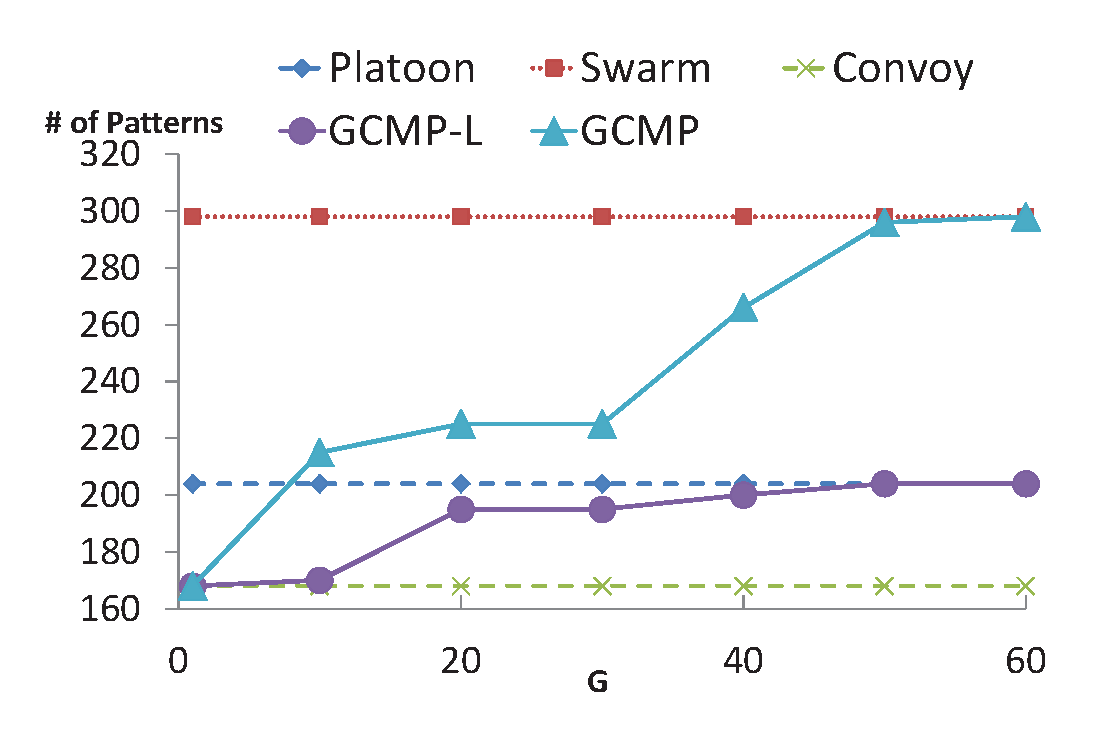
\includegraphics[width=\textwidth]{exp/effectiveness/effect_geolife.eps}
        \caption{Geolife}
    \end{subfigure}
    \begin{subfigure}[b]{0.33\textwidth}
        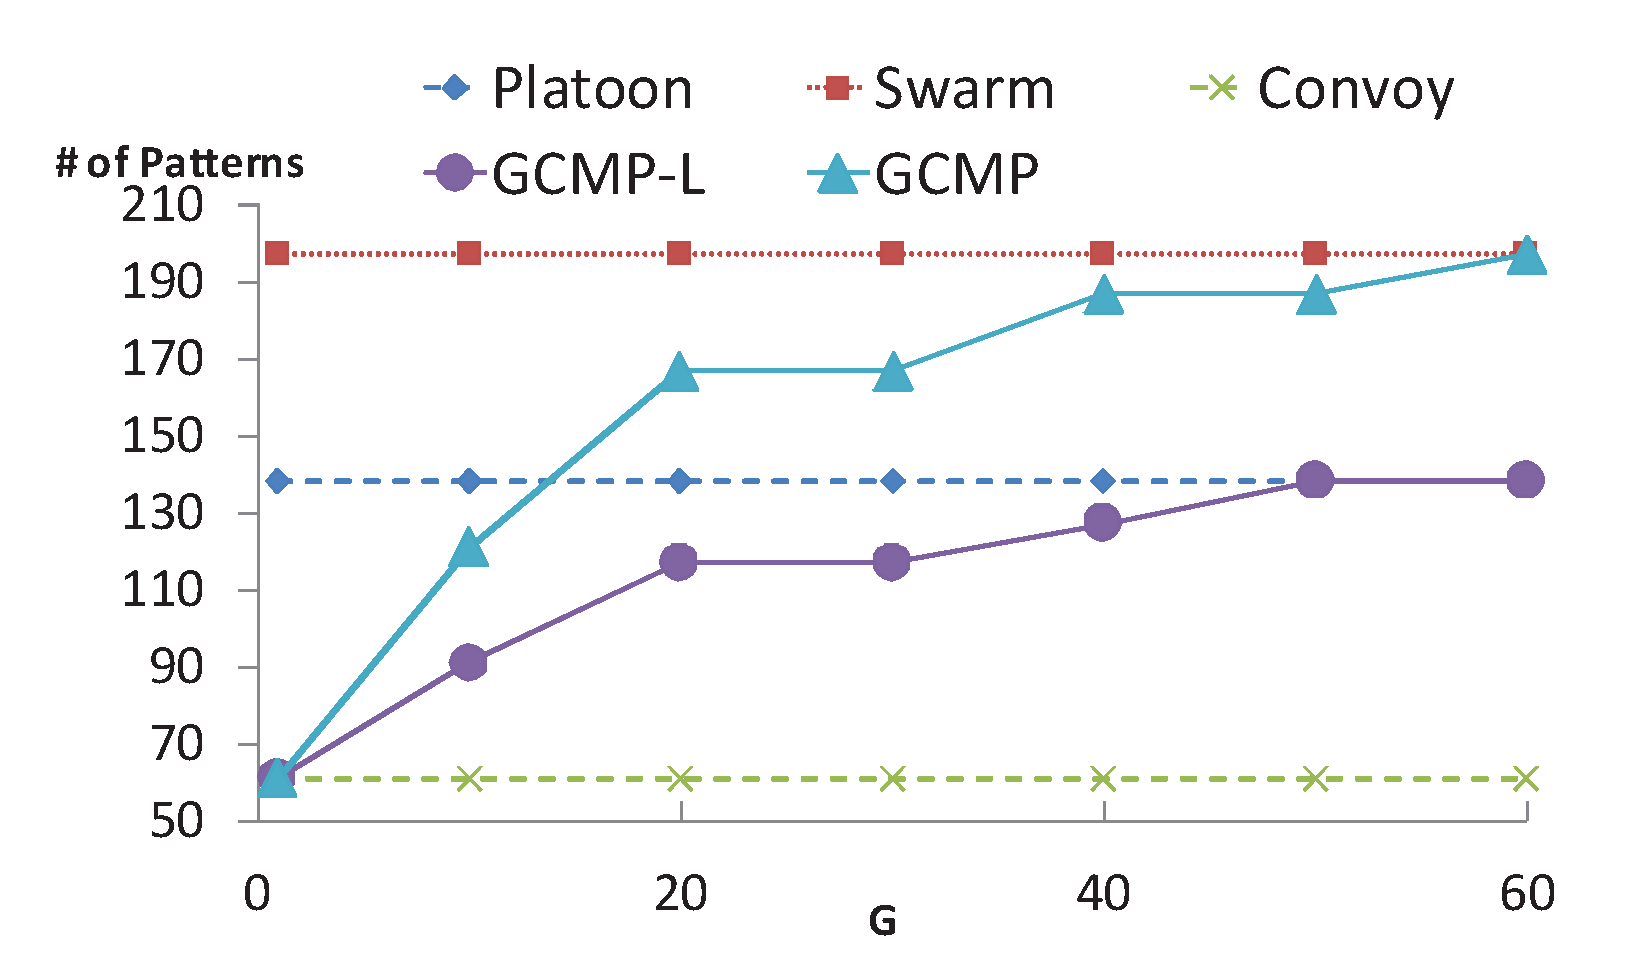
\includegraphics[width=\textwidth]{exp/effectiveness/effect_shopping.eps}
        \caption{ACTShopping}
    \end{subfigure}
    \begin{subfigure}[b]{0.3\textwidth}
        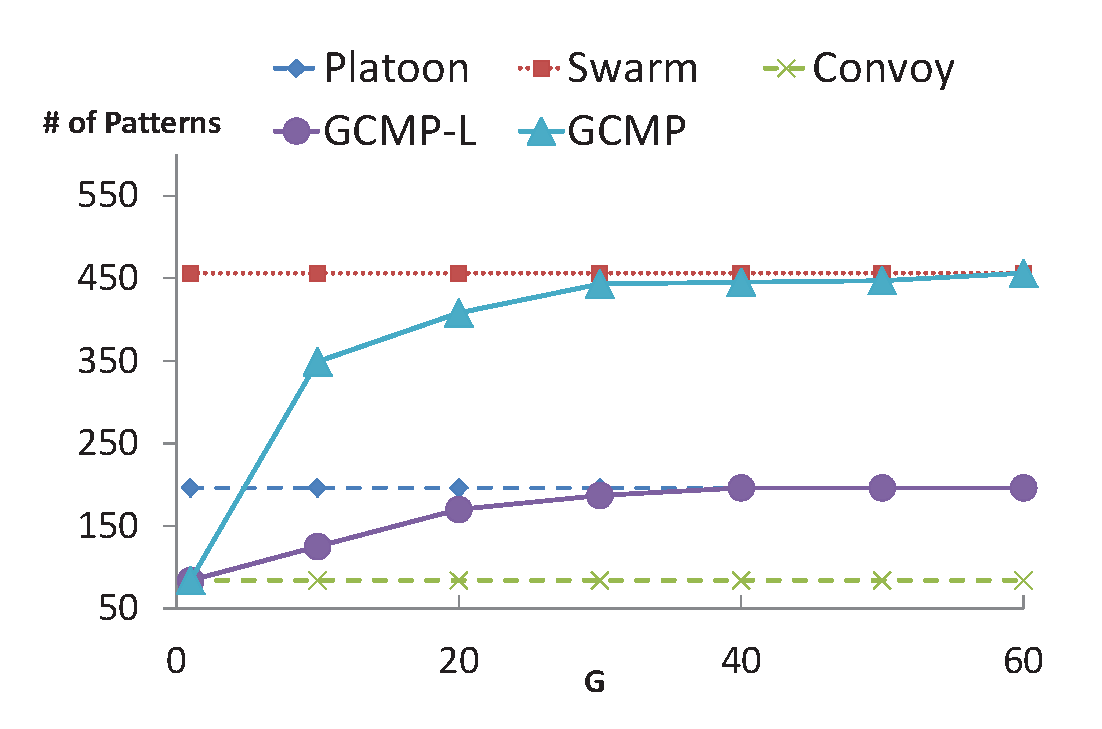
\includegraphics[width=\textwidth]{exp/effectiveness/effect_taxi.eps}
        \caption{SingTaxi}
    \end{subfigure}
\caption{Effectiveness of GCMP model on sampled datasets.}
\label{exp:effectiveness}
\end{figure*}


\subsection{Effects of $G$ on GCMP}
We study the effects of the gap parameter $G$ on discovering co-movement patterns. 
As shown in Figure~\ref{fig:related_work_scalability},
existing works are not able to handle large trajectories, we sample and cluster $1$ million  
trajectory points from the three real data. We use two instances of GCMPs, GCMP-L where the
$L$ value is default and GCMP where $L = 1$.  We measure the number
of patterns discvoered by different methods. The results are presented in Figure~\ref{exp:effectiveness}.

We can see from Figures~\ref{exp:effectiveness} that the number of patterns
discovered by GCMP is a positively related to $G$. When $G =1$, the number
of patterns returned by GCMP and GCMP-L are identical to \emph{convoy}. As $G$ grows,
the number returned by GCMP-L converges to \emph{platoon}. For example, in (a), two
patterns converge when $G$ is $40$. Similarly in (b) and (c), two patterns converge
when $G$ is $50$. The reason is that when $G$ is large enough,
 all consecutive segments in \emph{platoon} satisfy the $G$-connectivity. Similar
 trend applies between GCMP and \emph{swarm}. As see from the figures, in (a), two
 patterns converge at $G=50$; while in (b) and (c) the two patterns converge
 at $G=60$ and $G=40$ respectively. We further
 note that, existing patterns has different granularity in temporal domain. As we seen
 from the three figures, the number of \emph{swarm} is greater than \emph{platoon} and
 \emph{convoy}. Despite none of the existing patterns are able to fine-grain control
 the temporal domain of patterns, GCMP can discover the patterns more precisely. 
 These results confirms the usefulness of GCMP in expressing other patterns.
  



\subsection{Performance Comparison}
We now study the performance of our GCMP methods. We use TRPM as
the baseline algorithm and implement SPM and SPM+.

\begin{table}
\begin{tabular}{c|c|l}
\hline 
\textbf{Variables} & \textbf{Meaning} & \textbf{Values} \\ 
\hline 
M & min size of object set &  20, 40, \textbf{60},80,100 \\ 
\hline 
K & min duration & 60, 120, \textbf{180}, 240, 300 \\ 
\hline 
L & min local duration & 10, 20, \textbf{30}, 40,50 \\ 
\hline 
G & max gap & 5,10,\textbf{15},20,25 \\ 
\hline 
$\epsilon$ & DBSCAN parameter & 3,6,\textbf{9},12 \\ 
\hline 
minPt & DBSCAN parameter & 3,6,\textbf{9},12 \\ 
\hline 
\end{tabular} 
\caption{Pattern Parameters and their default values.}
\end{table}


\subsubsection{Effects of clusters $\epsilon$, minPt}
\subsubsection{Effects of pattern parameters $M,L,K,G$}


\subsection{SPM Analysis}
\subsubsection{Load Balance}
\subsubsection{Scalability}



